\newpage
\begin{center}
  \textbf{\large 1. ОТЧЁТ ЗА УЧЕБНУЮ ПРАКТИКУ}
\end{center}
\refstepcounter{chapter}
\addcontentsline{toc}{chapter}{1. ОТЧЁТ ЗА УЧЕБНУЮ ПРАКТИКУ}


\section{База данных AS-IS}

% В текущей архитектуре Keycloak (AS-IS) база данных содержит таблицы, связанные с управлением сессиями, аутентификацией и пользовательскими данными. Основными таблицами являются USER_SESSION, которая хранит активные сессии пользователей, CLIENT_SESSION, отслеживающая взаимодействие сессий с клиентами, и AUTHENTICATION_LOG, содержащая записи о событиях аутентификации, таких как успешные и неудачные попытки входа. OFFLINE_SESSION используется для хранения долгосрочных сессий, поддерживающих офлайн-доступ. Однако в данной модели отсутствует детализированное хранение истории сессий, данных об активности пользователя, механизмов обнаружения аномалий и управления сессиями на более глубоком уровне, что ограничивает возможности мониторинга и автоматического контроля за активностью пользователей.

% 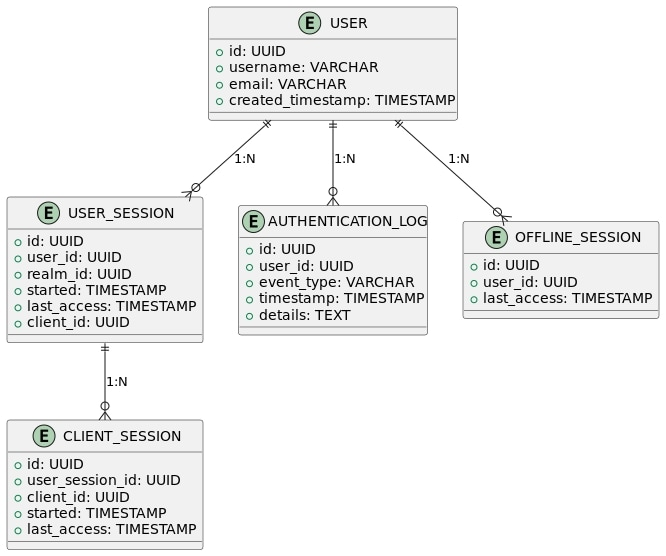
\includegraphics[width=\textwidth]{images/DB_AS-IS.jpg}

\section{База данных TO-BE}

% Обновленная архитектура (TO-BE) расширяет функциональность базы данных за счет новых таблиц, позволяющих вести детализированный учет сессий и анализировать поведение пользователей. Добавлены SESSION_HISTORY, которая фиксирует завершенные сессии и причины их завершения, ANOMALOUS_LOGINS для хранения данных о подозрительных входах, а также SESSION_EVENTS, регистрирующая ключевые события внутри сессий. USER_DEVICES отслеживает устройства, с которых пользователи входили в систему, а GEO_DATA_CACHE кэширует информацию о геолокации IP-адресов для ускоренного определения местоположения пользователей. Также добавлена LOGIN_ATTEMPTS для учета успешных и неудачных попыток входа и ADMIN_ACTIONS для логирования действий администраторов, связанных с управлением сессиями. Эти изменения позволяют реализовать аналитику активности пользователей, автоматически выявлять подозрительные входы и обеспечивать более высокий уровень безопасности при работе с Keycloak.

% 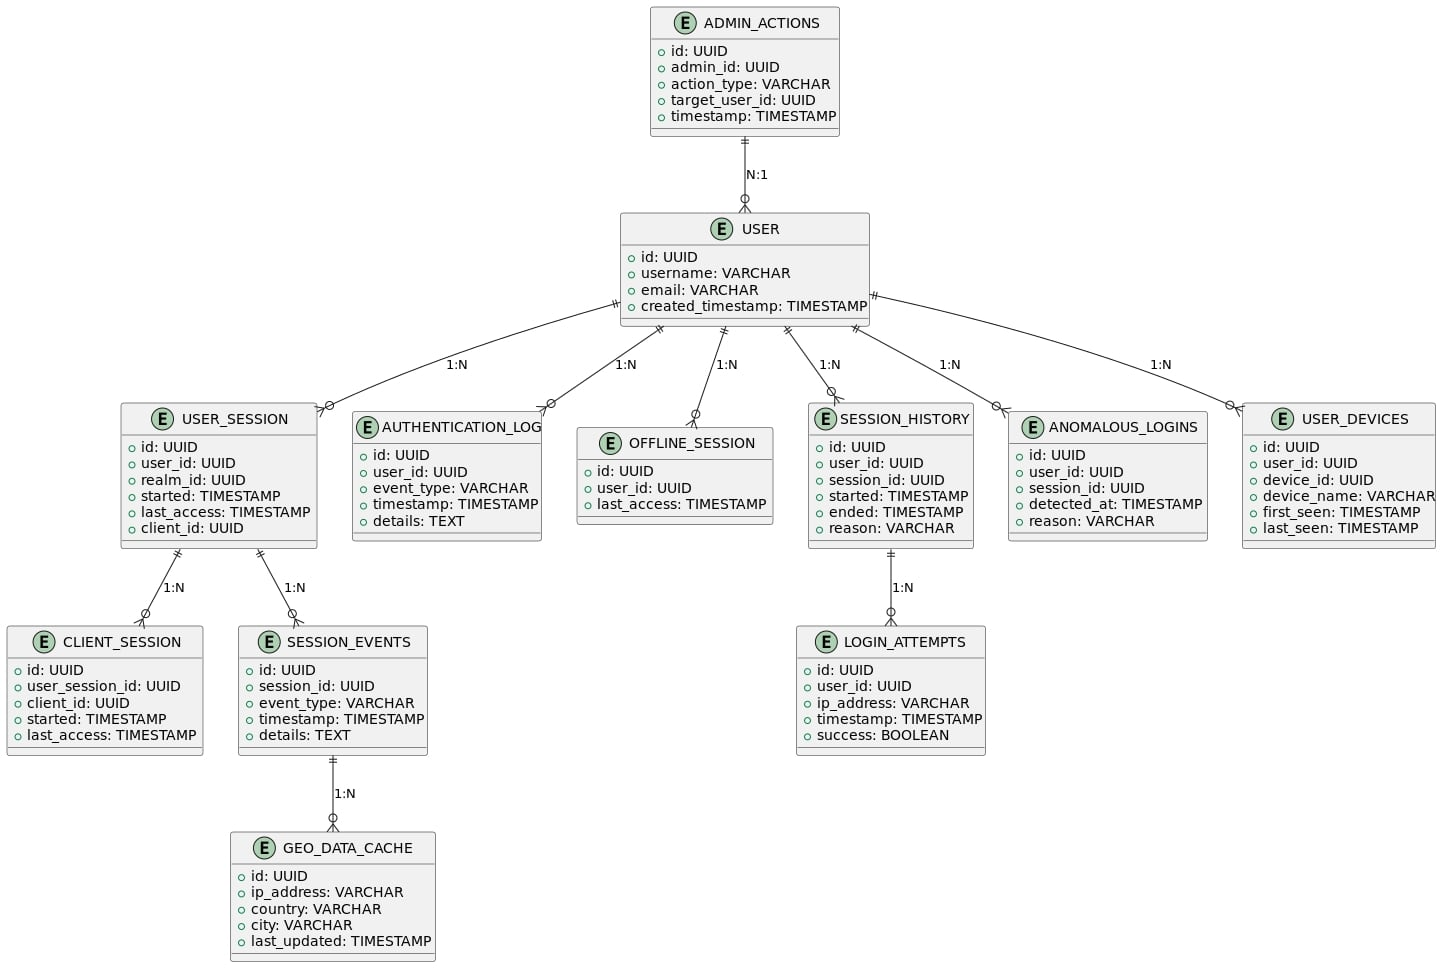
\includegraphics[width=\textwidth]{images/DB_TO-BE.jpg}

\section{Структура AS-IS}

% В текущей архитектуре Keycloak (AS-IS) компоненты системы включают стандартные модули аутентификации, управления сессиями и хранения данных пользователей. Authentication Module обрабатывает запросы на вход пользователей и передает управление в Session Management, который создает и отслеживает активные сессии, взаимодействуя с User Database для сохранения информации о пользователях и их активных сессиях. Администраторы управляют пользователями и сессиями через Admin Console, предоставляющую базовые возможности мониторинга. Однако в данной архитектуре отсутствует детальная аналитика сессий, система обнаружения аномальной активности, интеграция с внешними сервисами для анализа IP-адресов и возможность автоматического завершения неактивных или подозрительных сессий.

% 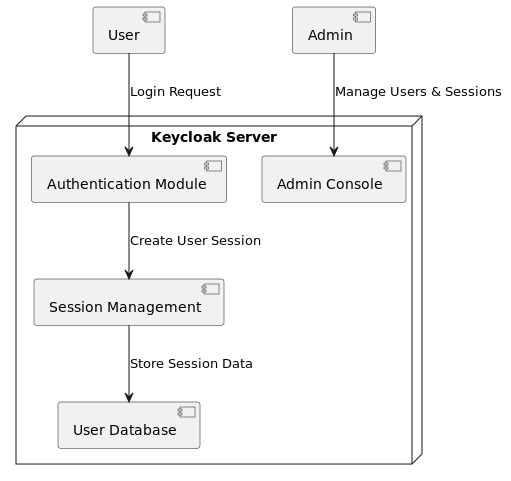
\includegraphics[width=\textwidth]{images/Arch_AS-IS.jpg}

\section{Структура TO-BE}

% Обновленная архитектура (TO-BE) дополняет базовый функционал Keycloak новым модулем Custom Session Management Module, включающим несколько специализированных компонентов. Session Analytics отвечает за сбор и визуализацию данных о сессиях, Anomaly Detection анализирует входы и выявляет подозрительную активность, а Session API предоставляет интерфейс для управления сессиями через программные вызовы. GeoIP Service интегрируется с внешним API для определения геолокации пользователей по IP-адресу, а Custom Session Database хранит дополнительные данные о сессиях, аномалиях и истории входов. Эти изменения позволяют администраторам получать детализированные отчеты о пользовательской активности, автоматически завершать неактивные сессии, а также оперативно реагировать на угрозы безопасности в системе.

% 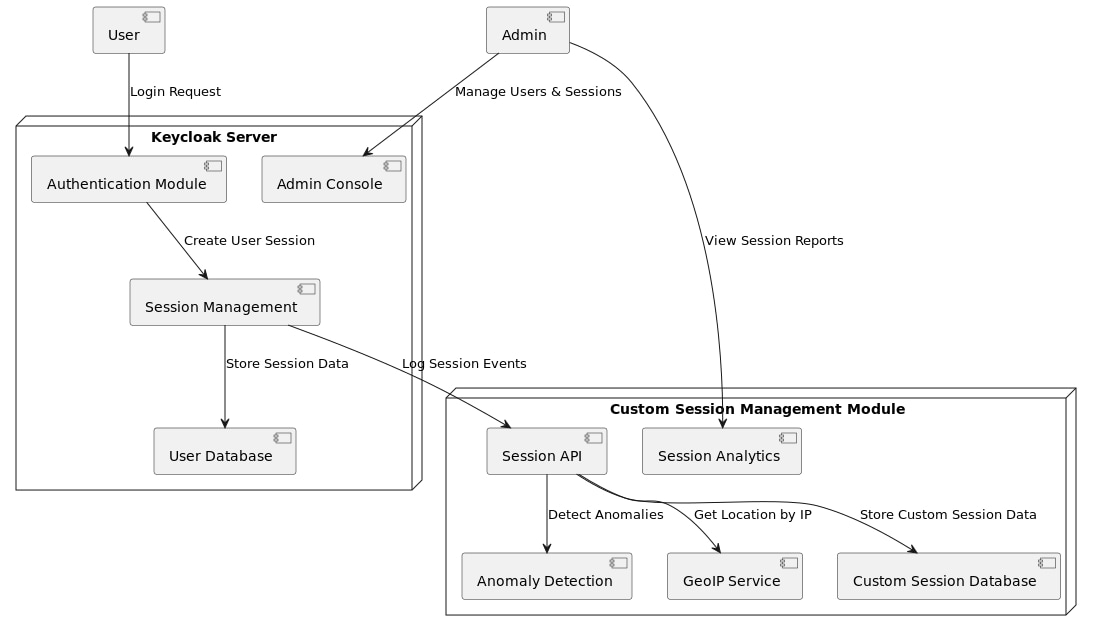
\includegraphics[width=\textwidth]{images/Arch_TO-BE.jpg}

\section{Алгоритм обнаружения аномалий}

% Алгоритм анализирует входы пользователей в систему для выявления подозрительных действий, таких как логин с нового устройства, входы с разных геолокаций за короткий промежуток времени или многократные попытки входа. При каждом входе система получает IP-адрес, геолокацию и информацию об устройстве, а затем сравнивает их с историческими данными. Если система фиксирует резкое изменение местоположения (например, вход из другой страны спустя несколько минут после предыдущего), использование нового устройства или слишком частые попытки входа, она присваивает событию уровень риска. В зависимости от настроек может быть выполнена автоматическая блокировка учетной записи, отправлено уведомление пользователю или администратору, а также записано предупреждение в журнал аномалий. Для повышения точности применяются эвристические методы, учитывающие тип пользователя, его предыдущие действия и возможные VPN-соединения.

% 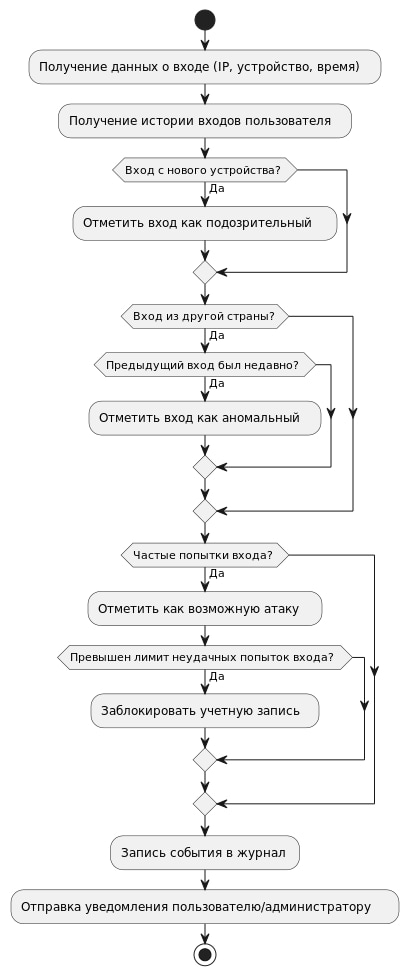
\includegraphics[width=\textwidth]{images/SearchAnom.jpg}

\section{Алгоритм завершения сессий}

% Алгоритм предназначен для автоматического завершения пользовательских сессий, которые остаются неактивными дольше заданного времени или превышают установленный лимит жизни. В фоновом режиме периодически выполняется проверка всех активных сессий, где анализируется время последней активности и текущее состояние пользователя. Если система фиксирует бездействие, превышающее установленный порог, или истечение максимального времени жизни сессии, она автоматически завершает её, записывая событие в журнал активности. В случае необходимости пользователю может быть отправлено уведомление с предупреждением о разлогинивании. Такой механизм помогает предотвратить захват неиспользуемых сессий злоумышленниками, а также повышает общую безопасность системы, особенно в корпоративных и финансовых средах.

% 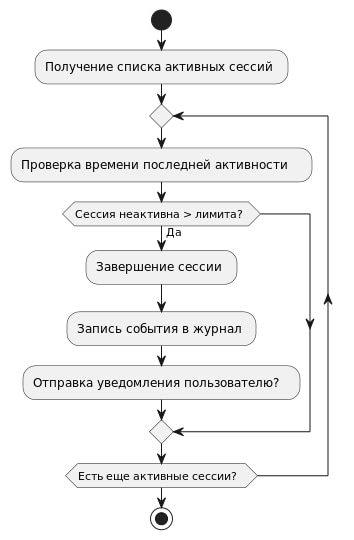
\includegraphics[width=\textwidth]{images/Autoend.jpg}